% Latin Modern labels
% Made with Xematics. Positions are in px (1 px = 0.75 pt), as in the SVG export.
\documentclass[tikz, border=4pt]{standalone}
\usepackage[T1]{fontenc}
\usepackage{lmodern}
\usepackage{amsmath, amssymb}
\definecolor{xm1}{HTML}{FFFFFF}
\definecolor{xm2}{HTML}{D4E8F5}
\definecolor{xm3}{HTML}{0072B2}
\definecolor{xm4}{HTML}{F1F2F4}
\definecolor{xm5}{HTML}{4B5563}
\definecolor{xm6}{HTML}{FBE8C4}
\definecolor{xm7}{HTML}{B97800}
\definecolor{xm8}{HTML}{B8C0CC}
\definecolor{xm9}{HTML}{1F2937}
\definecolor{xm10}{HTML}{6B7280}
\begin{document}
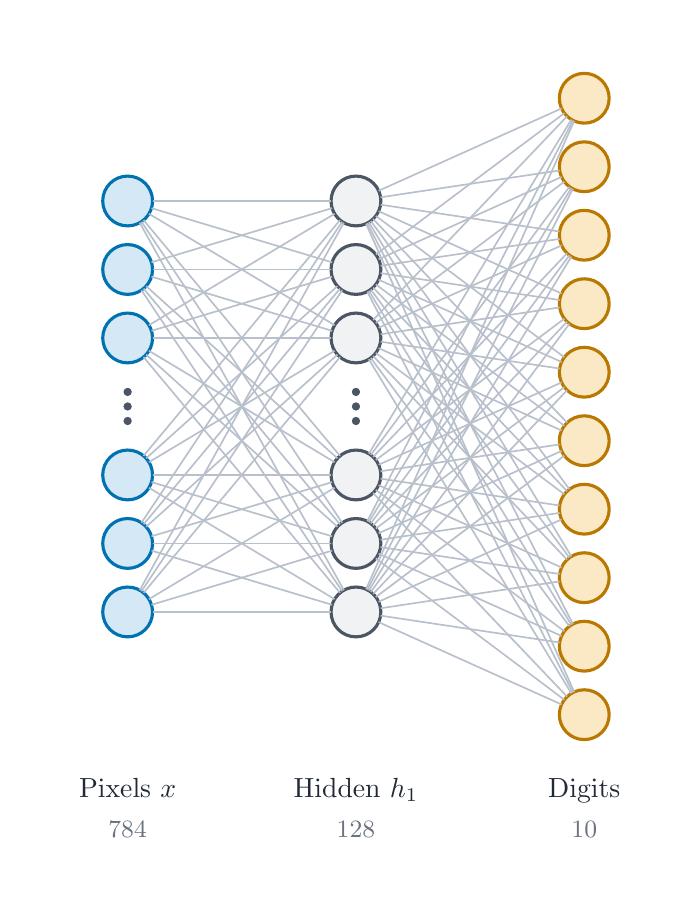
\begin{tikzpicture}[x=0.75pt, y=-0.75pt]
  \tikzset{
    xm input/.style={circle, minimum size=18pt, inner sep=0, outer sep=0, fill=xm2, draw=xm3, line width=1.13pt},
    xm hidden/.style={circle, minimum size=18pt, inner sep=0, outer sep=0, fill=xm4, draw=xm5, line width=1.13pt},
    xm output/.style={circle, minimum size=18pt, inner sep=0, outer sep=0, fill=xm6, draw=xm7, line width=1.13pt},
    xm edge/.style={draw=xm8, line width=0.6pt},
    xm dots/.style={fill=xm5},
    xm name xm9/.style={text=xm9, inner sep=0, font=\rmfamily\fontsize{9.75}{11.7}\selectfont},
    xm size xm10/.style={text=xm10, inner sep=0, font=\rmfamily\fontsize{9}{10.8}\selectfont},
  }
  \fill[xm1] (0,0) rectangle (309.63,415.57);
  % Neurons
  \node[xm input] (n-0-0) at (48.16,83.5) {};
  \node[xm input] (n-0-1) at (48.16,116.5) {};
  \node[xm input] (n-0-2) at (48.16,149.5) {};
  \node[xm input] (n-0-781) at (48.16,215.5) {};
  \node[xm input] (n-0-782) at (48.16,248.5) {};
  \node[xm input] (n-0-783) at (48.16,281.5) {};
  \node[xm hidden] (n-1-0) at (158.16,83.5) {};
  \node[xm hidden] (n-1-1) at (158.16,116.5) {};
  \node[xm hidden] (n-1-2) at (158.16,149.5) {};
  \node[xm hidden] (n-1-125) at (158.16,215.5) {};
  \node[xm hidden] (n-1-126) at (158.16,248.5) {};
  \node[xm hidden] (n-1-127) at (158.16,281.5) {};
  \node[xm output] (n-2-0) at (268.16,34) {};
  \node[xm output] (n-2-1) at (268.16,67) {};
  \node[xm output] (n-2-2) at (268.16,100) {};
  \node[xm output] (n-2-3) at (268.16,133) {};
  \node[xm output] (n-2-4) at (268.16,166) {};
  \node[xm output] (n-2-5) at (268.16,199) {};
  \node[xm output] (n-2-6) at (268.16,232) {};
  \node[xm output] (n-2-7) at (268.16,265) {};
  \node[xm output] (n-2-8) at (268.16,298) {};
  \node[xm output] (n-2-9) at (268.16,331) {};
  % Connections 0
  \draw[xm edge] (n-0-0) -- (n-1-0);
  \draw[xm edge] (n-0-0) -- (n-1-1);
  \draw[xm edge] (n-0-0) -- (n-1-2);
  \draw[xm edge] (n-0-0) -- (n-1-125);
  \draw[xm edge] (n-0-0) -- (n-1-126);
  \draw[xm edge] (n-0-0) -- (n-1-127);
  \draw[xm edge] (n-0-1) -- (n-1-0);
  \draw[xm edge] (n-0-1) -- (n-1-1);
  \draw[xm edge] (n-0-1) -- (n-1-2);
  \draw[xm edge] (n-0-1) -- (n-1-125);
  \draw[xm edge] (n-0-1) -- (n-1-126);
  \draw[xm edge] (n-0-1) -- (n-1-127);
  \draw[xm edge] (n-0-2) -- (n-1-0);
  \draw[xm edge] (n-0-2) -- (n-1-1);
  \draw[xm edge] (n-0-2) -- (n-1-2);
  \draw[xm edge] (n-0-2) -- (n-1-125);
  \draw[xm edge] (n-0-2) -- (n-1-126);
  \draw[xm edge] (n-0-2) -- (n-1-127);
  \draw[xm edge] (n-0-781) -- (n-1-0);
  \draw[xm edge] (n-0-781) -- (n-1-1);
  \draw[xm edge] (n-0-781) -- (n-1-2);
  \draw[xm edge] (n-0-781) -- (n-1-125);
  \draw[xm edge] (n-0-781) -- (n-1-126);
  \draw[xm edge] (n-0-781) -- (n-1-127);
  \draw[xm edge] (n-0-782) -- (n-1-0);
  \draw[xm edge] (n-0-782) -- (n-1-1);
  \draw[xm edge] (n-0-782) -- (n-1-2);
  \draw[xm edge] (n-0-782) -- (n-1-125);
  \draw[xm edge] (n-0-782) -- (n-1-126);
  \draw[xm edge] (n-0-782) -- (n-1-127);
  \draw[xm edge] (n-0-783) -- (n-1-0);
  \draw[xm edge] (n-0-783) -- (n-1-1);
  \draw[xm edge] (n-0-783) -- (n-1-2);
  \draw[xm edge] (n-0-783) -- (n-1-125);
  \draw[xm edge] (n-0-783) -- (n-1-126);
  \draw[xm edge] (n-0-783) -- (n-1-127);
  % Connections 1
  \draw[xm edge] (n-1-0) -- (n-2-0);
  \draw[xm edge] (n-1-0) -- (n-2-1);
  \draw[xm edge] (n-1-0) -- (n-2-2);
  \draw[xm edge] (n-1-0) -- (n-2-3);
  \draw[xm edge] (n-1-0) -- (n-2-4);
  \draw[xm edge] (n-1-0) -- (n-2-5);
  \draw[xm edge] (n-1-0) -- (n-2-6);
  \draw[xm edge] (n-1-0) -- (n-2-7);
  \draw[xm edge] (n-1-0) -- (n-2-8);
  \draw[xm edge] (n-1-0) -- (n-2-9);
  \draw[xm edge] (n-1-1) -- (n-2-0);
  \draw[xm edge] (n-1-1) -- (n-2-1);
  \draw[xm edge] (n-1-1) -- (n-2-2);
  \draw[xm edge] (n-1-1) -- (n-2-3);
  \draw[xm edge] (n-1-1) -- (n-2-4);
  \draw[xm edge] (n-1-1) -- (n-2-5);
  \draw[xm edge] (n-1-1) -- (n-2-6);
  \draw[xm edge] (n-1-1) -- (n-2-7);
  \draw[xm edge] (n-1-1) -- (n-2-8);
  \draw[xm edge] (n-1-1) -- (n-2-9);
  \draw[xm edge] (n-1-2) -- (n-2-0);
  \draw[xm edge] (n-1-2) -- (n-2-1);
  \draw[xm edge] (n-1-2) -- (n-2-2);
  \draw[xm edge] (n-1-2) -- (n-2-3);
  \draw[xm edge] (n-1-2) -- (n-2-4);
  \draw[xm edge] (n-1-2) -- (n-2-5);
  \draw[xm edge] (n-1-2) -- (n-2-6);
  \draw[xm edge] (n-1-2) -- (n-2-7);
  \draw[xm edge] (n-1-2) -- (n-2-8);
  \draw[xm edge] (n-1-2) -- (n-2-9);
  \draw[xm edge] (n-1-125) -- (n-2-0);
  \draw[xm edge] (n-1-125) -- (n-2-1);
  \draw[xm edge] (n-1-125) -- (n-2-2);
  \draw[xm edge] (n-1-125) -- (n-2-3);
  \draw[xm edge] (n-1-125) -- (n-2-4);
  \draw[xm edge] (n-1-125) -- (n-2-5);
  \draw[xm edge] (n-1-125) -- (n-2-6);
  \draw[xm edge] (n-1-125) -- (n-2-7);
  \draw[xm edge] (n-1-125) -- (n-2-8);
  \draw[xm edge] (n-1-125) -- (n-2-9);
  \draw[xm edge] (n-1-126) -- (n-2-0);
  \draw[xm edge] (n-1-126) -- (n-2-1);
  \draw[xm edge] (n-1-126) -- (n-2-2);
  \draw[xm edge] (n-1-126) -- (n-2-3);
  \draw[xm edge] (n-1-126) -- (n-2-4);
  \draw[xm edge] (n-1-126) -- (n-2-5);
  \draw[xm edge] (n-1-126) -- (n-2-6);
  \draw[xm edge] (n-1-126) -- (n-2-7);
  \draw[xm edge] (n-1-126) -- (n-2-8);
  \draw[xm edge] (n-1-126) -- (n-2-9);
  \draw[xm edge] (n-1-127) -- (n-2-0);
  \draw[xm edge] (n-1-127) -- (n-2-1);
  \draw[xm edge] (n-1-127) -- (n-2-2);
  \draw[xm edge] (n-1-127) -- (n-2-3);
  \draw[xm edge] (n-1-127) -- (n-2-4);
  \draw[xm edge] (n-1-127) -- (n-2-5);
  \draw[xm edge] (n-1-127) -- (n-2-6);
  \draw[xm edge] (n-1-127) -- (n-2-7);
  \draw[xm edge] (n-1-127) -- (n-2-8);
  \draw[xm edge] (n-1-127) -- (n-2-9);
  % Layers
  \fill[xm dots] (48.16,175.5) circle[radius=2];
  \fill[xm dots] (48.16,182.5) circle[radius=2];
  \fill[xm dots] (48.16,189.5) circle[radius=2];
  \fill[xm dots] (158.16,175.5) circle[radius=2];
  \fill[xm dots] (158.16,182.5) circle[radius=2];
  \fill[xm dots] (158.16,189.5) circle[radius=2];
  % Labels
  \node[xm name xm9, anchor=base] at (48.16,370.73) {Pixels $x$};
  \node[xm size xm10, anchor=base] at (48.16,390.09) {784};
  \node[xm name xm9, anchor=base] at (158.16,370.73) {Hidden $h_1$};
  \node[xm size xm10, anchor=base] at (158.16,390.09) {128};
  \node[xm name xm9, anchor=base] at (268.16,370.73) {Digits};
  \node[xm size xm10, anchor=base] at (268.16,390.09) {10};
\end{tikzpicture}
\end{document}
